%%
%% Copyright 2026 Elsevier Ltd
%%
%% This file is part of the 'Elsarticle Bundle'.
%% ---------------------------------------------
%%
%% It may be distributed under the conditions of the LaTeX Project Public
%% License, either version 1.2 of this license or (at your option) any
%% later version.  The latest version of this license is in
%%    http://www.latex-project.org/lppl.txt
%% and version 1.2 or later is part of all distributions of LaTeX
%% version 1999/12/01 or later.
%%
%% The list of all files belonging to the 'Elsarticle Bundle' is
%% given in the file `manifest.txt'.
%%

%% Template article for Elsevier's document class `elsarticle'
%% with numbered style bibliographic references
%% SP 2008/03/01

\documentclass[preprint,12pt, a4paper]{elsarticle}

%% Use the option review to obtain double line spacing
%% \documentclass[authoryear,preprint,review,12pt]{elsarticle}

%% For including figures, graphicx.sty has been loaded in
%% elsarticle.cls. If you prefer to use the old commands
%% please give \usepackage{epsfig}

%% The amssymb package provides various useful mathematical symbols
\usepackage{amssymb}
\usepackage{hyperref}
\setlength{\parindent}{0pt}
%% The amsthm package provides extended theorem environments
%% \usepackage{amsthm}

\journal{SoftwareX}

\begin{document}
\renewcommand{\labelenumii}{\arabic{enumi}.\arabic{enumii}}

\begin{frontmatter}

\title{libMesh: A C++ Library for Finite Element and Finite Volume Based Multiphysics}

\author[inl]{Roy H. Stogner}
\author[akselos]{John W. Peterson}
\author[inl]{Alexander D. Lindsay}
\author[akselos]{David J. Knezevic}
\author[hartree]{Nuno Nobre}
\author[inl]{Logan Harbour}
\author[inl]{Guillaume L. Giudicelli}
\author[inl]{Derek R. Gaston}
\author[inl]{Cody J. Permann}
\author[ub]{Paul T. Bauman}
\author[inlcmm]{Daniel Schwen}
\author[inl]{Patrick Behne}
\author[ut]{Benjamin Kirk}

\address[inl]{Computational Frameworks, Idaho National Laboratory, Idaho Falls, ID 83415, USA}
\address[akselos]{Akselos}
\address[hartree]{Hartree Centre, Science and Technology Facilities Council (STFC), UK}
\address[ub]{University at Buffalo, Department of Mechanical and Aerospace Engineering, Buffalo, NY, USA}
\address[inlcmm]{Computational Mechanics and Materials, Idaho National Laboratory, Idaho Falls, ID 83415, USA}
\address[ut]{Department of Aerospace Engineering and Engineering Mechanics (ASE), University of Texas at Austin, Austin, TX, USA}

\begin{abstract}
libMesh is an open-source C++ library for parallel, spatially adaptive finite element and finite
volume simulation, last described in detail in 2006. Since then, the library has added
hybridizable discontinuous Galerkin and other statically condensable discretizations; isogeometric
analysis with rational bases and arbitrary B\'ezier extraction operators for trimmed geometry;
native polyhedral elements; and TIMPI, a standalone parallel communication submodule implementing
modern nonblocking-exchange algorithms. Automatic differentiation, certified reduced-basis model
order reduction, and adjoint-driven $hp$-adaptivity round out the expanded numerical toolkit. This
article surveys these capabilities and the multiphysics applications they enable.
\end{abstract}

\begin{keyword}
finite elements \sep finite volume \sep parallel computing \sep isogeometric analysis \sep multiphysics \sep adaptive mesh refinement
\end{keyword}

\end{frontmatter}

\section*{Required Metadata}

\section*{Current code version}

\begin{table}[!h]
\begin{tabular}{|l|p{6.5cm}|p{6.5cm}|}
\hline
\textbf{Nr.} & \textbf{Code metadata description} & \textbf{Metadata} \\
\hline
C1 & Current code version & v1.9.0 development series (confirm exact tag at submission) \\
\hline
C2 & Permanent GitHub link to code/repository used for this code version & \url{https://github.com/libMesh/libmesh} \\
\hline
C3 & Legal Code License & GNU Lesser General Public License v2.1 (LGPL-2.1) \\
\hline
C4 & Code versioning system used & git (hosted on GitHub) \\
\hline
C5 & Software code languages, tools, and services used & C++ (C++17); MPI; PETSc/SLEPc (optional); TIMPI (bundled, required); MetaPhysicL (bundled, optional); Eigen; TetGen, Netgen, Triangle (bundled); ExodusII/SEACAS; NetCDF; VTK \\
\hline
C6 & Compilation requirements, operating environments \& dependencies & Autoconf/Automake build (\texttt{configure} \& \texttt{make}); C++17 compiler; MPI implementation (no supported build configuration omits it in practice); TIMPI submodule (required); PETSc strongly recommended for solvers and static condensation \\
\hline
C7 & If available Link to developer documentation/manual & \url{https://libmesh.github.io/} \\
\hline
C8 & Support email for questions & \url{https://github.com/libmesh/libmesh/discussions} \\
\hline
\end{tabular}
\caption{Code metadata (mandatory)}
\label{tab:metadata}
\end{table}

\begin{enumerate}

\item Motivation and significance

libMesh is an open-source C++ library providing general, physics-independent infrastructure for
parallel, spatially adaptive finite element -- and, increasingly, finite volume -- simulation. Its
2006 description~\cite{kirk2006libmesh} covered a mesh and degree-of-freedom data model,
$h$-adaptive refinement and coarsening with hanging-node constraints, and a domain-decomposition
parallel model built atop third-party solver libraries such as PETSc. That core design still
holds, but nearly every capability surveyed here postdates it.

libMesh has been under continuous development for the twenty years since, accumulating tens of
thousands of commits from a broad developer community. Its applications now require
discretizations and geometric representations unavailable in 2006: hybridizable and other
statically condensed formulations suited to advection-dominated transport; isogeometric meshes
derived from trimmed or piecewise-rational-spline CAD geometry; and general polyhedral cells, which
suit finite-volume-style discretizations far better than the fixed simplicial and tensor-product
elements previously available. The parallel communication layer has also been substantially
reworked, and new infrastructure has been added for automatic differentiation, certified
reduced-order modeling, and goal-oriented adaptivity.

Two largely independent application communities motivate and use these capabilities. The MOOSE
multiphysics framework~\cite{permann2020moose}, developed at Idaho National Laboratory (INL),
relies on libMesh for its finite element capabilities and, through the discontinuous/monomial
discretizations and generalized ghosting infrastructure described in Section 2, for its
finite-volume-style capabilities. MOOSE underpins INL's fission and fusion reactor multiphysics
work, and a comparable MOOSE-based fusion-device effort is under way in the UK, where the Hartree
Centre (STFC) collaborates closely with the UK Atomic Energy Authority. Independently of MOOSE,
Akselos builds commercial reduced-order-modeling and digital-twin engineering-analysis products
directly on libMesh's certified reduced-basis infrastructure. This article surveys the
library-level capabilities underlying both communities.

\item Software description

\begin{enumerate}

\item Software architecture

libMesh is organized around a small set of deliberately physics-independent core abstractions:
\texttt{Mesh}, \texttt{Elem}, \texttt{DofMap}, \texttt{System}, and the finite element
(\texttt{FEBase}) classes. An application supplies the equations; libMesh supplies mesh
management, degree-of-freedom numbering, adaptivity, and parallel communication. The capabilities
described below extend this architecture without replacing it: new finite element families,
element types, and mesh constructs plug into the existing \texttt{FEBase}/\texttt{Elem} hierarchy;
new solver and preconditioning machinery plugs into the existing \texttt{System}/\texttt{DofMap}
interfaces; and new parallel primitives are exposed through the bundled TIMPI submodule.

\item Software functionalities

\textbf{Discretizations for finite element and finite volume multiphysics.} The
\texttt{StaticCondensation}, \texttt{StaticCondensationDofMap}, and
\texttt{StaticCondensationPreconditioner} classes implement hybridization and static condensation:
they assemble the full elemental system, then eliminate element-local degrees of freedom through a
local Schur complement before the global solve, using Eigen for the local dense factorizations.
Paired with the \texttt{SIDE\_HIERARCHIC} finite element family, which represents variables on
element facets, this supports hybridizable discontinuous Galerkin (HDG) discretizations for general
transport problems, including the advection-dominated regimes in which downstream MOOSE-based
applications use HDG.

General polyhedral cells are supported natively through the \texttt{Polyhedron} and
\texttt{C0Polyhedron} classes, whose topology (number of faces, sides, and nodes) is determined at
run time; libMesh's traditional hexahedral, tetrahedral, and prismatic elements fix their topology
at compile time. Polyhedral cells, including coarse cells formed by merging groups of finer
elements, match finite-volume-style stencils substantially better than fixed simplicial elements.
More broadly, finite-volume-style discretizations are enabled by libMesh's discontinuous/monomial
finite element spaces together with a generalized ghosting-functor framework
(\texttt{GhostingFunctor} and its specializations for point-neighbor, overlap, non-manifold, and
sibling coupling). This framework lets an application declare exactly which off-element data a
cell-centered discretization needs, so libMesh requires no dedicated finite-volume module.

\textbf{Isogeometric analysis.} The \texttt{RATIONAL\_BERNSTEIN} finite element family reweights
Bernstein/B\'ezier shape functions with per-node NURBS weights, giving the rational basis used in
isogeometric analysis (IGA)~\cite{hughes2005iga}. A corresponding element mapping type applies the
same rational representation to the geometric map itself, so meshes derived from
piecewise-rational-spline CAD geometry are represented exactly. Arbitrary B\'ezier extraction
operators~\cite{borden2011extraction}, needed when a structured IGA mesh is impractical to generate
automatically (as with trimmed geometry), reuse libMesh's generic linear-constraint infrastructure:
extraction coefficients read from ExodusII files are stored as constraint rows relating
spline-basis degrees of freedom to element-local nodes, so no IGA-specific parallel code path is
required.

\textbf{Meshing and I/O.} The \texttt{MeshTetInterface} abstract base class unifies libMesh's
interfaces to the bundled TetGen and Netgen tetrahedralizers, giving applications a single API for
generating volume meshes from boundary surfaces. Mesh I/O has expanded well beyond the 2006
formats to include extended ExodusII/Nemesis, VTK, Abaqus, and NetCDF support. The element library
has added high-order and shell element types, along with generic element-quality metrics (aspect
ratio, minimum/maximum angle, and scaled Jacobian).

\textbf{Parallel infrastructure.} Parallel communication is now implemented in TIMPI, a required
dependency that began as libMesh-internal code and was split into its own independently versioned
and tested repository in 2019. TIMPI offers interchangeable strategies for push/pull-style parallel
data exchange, selected through the \texttt{SyncType} enumeration (\texttt{NBX},
\texttt{ALLTOALL\_COUNTS}, \texttt{SENDRECEIVE}). The \texttt{NBX} strategy implements the
nonblocking dynamic sparse data exchange algorithm of Hoefler et al.~\cite{hoefler2010nbx}, which
avoids the all-to-all communication and a priori knowledge of message counts that earlier, simpler
schemes required.

\textbf{Numerics and solvers.} libMesh's generic numeric types (\texttt{TypeVector},
\texttt{TypeTensor}, \texttt{VectorValue}, \texttt{TensorValue}, \texttt{DenseVector}, and
\texttt{DenseMatrix}) are templated to work transparently with the dual-number type from the
bundled MetaPhysicL submodule. Downstream codes, notably MOOSE~\cite{lindsay2021metaphysicl}, can
therefore build exact-derivative Jacobian assembly on libMesh without any
automatic-differentiation-specific code path in libMesh itself. The certified reduced-basis model
order reduction capability -- offline/online reduced-basis construction, the empirical
interpolation method for nonaffine operators, and the successive constraint method for
stability-factor lower bounds -- is the numerical core of Akselos's commercial
reduced-order-modeling products. Finally, adjoint-based, goal-oriented error estimation and
$hp$-adaptive refinement strategies extend the flux-jump and patch-recovery indicators available
in 2006 to quantity-of-interest-driven adaptivity.

\item Sample code snippets analysis

The following excerpt, adapted from libMesh's HDG example driver, shows how a hybridized
discretization is declared. An element-interior vector unknown, its scalar components, facet
Lagrange multipliers (\texttt{SIDE\_HIERARCHIC}), and a global scalar constraint are added as
ordinary \texttt{System} variables; the \texttt{StaticCondensation} matrix class is then attached
to eliminate the element-interior unknowns before the global solve:

\begin{verbatim}
system.add_variable("qu", FIRST, L2_LAGRANGE_VEC);
system.add_variable("vel_x", FIRST, L2_LAGRANGE);
system.add_variable("lm_u", FIRST, SIDE_HIERARCHIC);
system.add_variable("lm_v", FIRST, SIDE_HIERARCHIC);
system.add_variable("pressure", FIRST, L2_LAGRANGE);
system.add_variable("global_lm", FIRST, SCALAR);
\end{verbatim}

Running this system in parallel requires no new solver, assembly, or communication code: the
\texttt{DofMap}, ghosting, and TIMPI-based infrastructure used by conventional continuous finite
element systems applies directly.

\end{enumerate}

\item Illustrative examples

libMesh's \texttt{examples/} tree includes runnable drivers that exercise these capabilities end to
end; the test suite covers capabilities that lack a dedicated example. Table~\ref{tab:examples}
lists a representative driver or test for each capability surveyed in Section 2.

\texttt{examples/vector\_fe/vector\_fe\_ex9} solves a Stokes-like vector transport problem with the
HDG formulation of Section 2.2: element-interior velocity and pressure unknowns are coupled to
facet Lagrange multipliers (\texttt{SIDE\_HIERARCHIC} variables), and \texttt{StaticCondensation}
eliminates the interior unknowns before the global, facet-only system is solved.
Figure~\ref{fig:hdg} shows the resulting lid-driven-cavity velocity streamlines, colored by speed,
with the expected primary recirculation vortex.

\begin{figure}[!h]
\centering
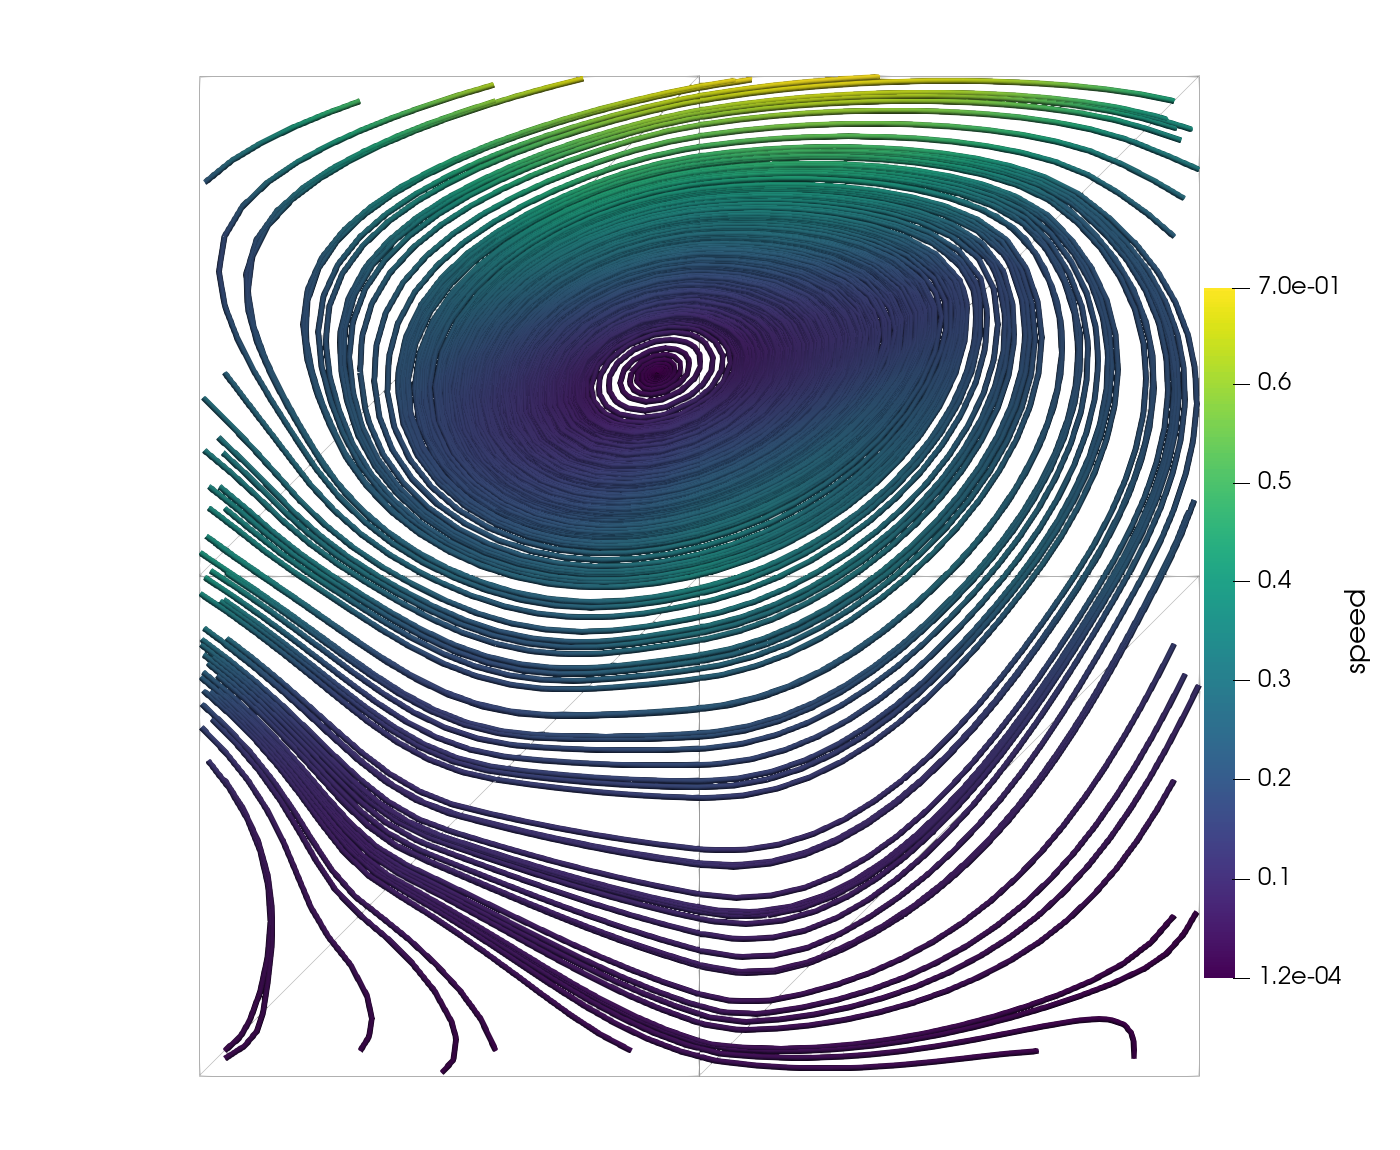
\includegraphics[width=0.55\textwidth]{figures/vector_fe_ex9_streamlines.png}
\caption{Velocity streamlines, colored by speed, for the HDG cavity-flow problem solved by
\texttt{examples/vector\_fe/vector\_fe\_ex9}, after static condensation of the element-interior
velocity/pressure unknowns.}
\label{fig:hdg}
\end{figure}

A minimal driver in the spirit of \texttt{examples/miscellaneous/miscellaneous\_ex6} illustrates
the unified tetrahedralization interface: it attaches a cube-shaped hole to a cubic domain and
passes both to \texttt{NetGenMeshInterface}, a \texttt{MeshTetInterface} subclass, to produce a
quality-constrained volume mesh. Figure~\ref{fig:mesh} shows a clipped view of the result, with
the interior hole and the surrounding fill both visible. The calling code works unchanged with
\texttt{TetGenMeshInterface} in place of the Netgen backend, which is precisely the uniformity
\texttt{MeshTetInterface} is meant to provide.

\begin{figure}[!h]
\centering
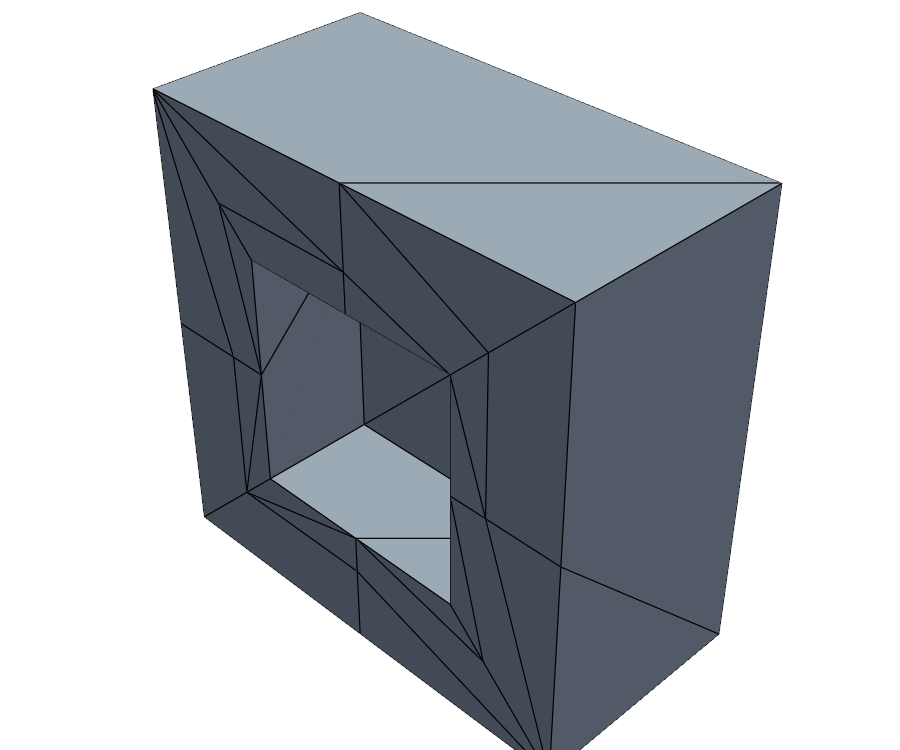
\includegraphics[width=0.55\textwidth]{figures/netgen_hole_demo.png}
\caption{Clipped view of a tetrahedralized cubic domain with a cube-shaped interior hole, generated
via \texttt{MeshTetInterface}'s Netgen backend.}
\label{fig:mesh}
\end{figure}

\begin{table}[!h]
\begin{tabular}{|p{4.3cm}|p{8.7cm}|}
\hline
\textbf{Capability} & \textbf{Runnable example or test} \\
\hline
Hybridization / static condensation (HDG) & \texttt{examples/vector\_fe/vector\_fe\_ex9} \\
\hline
Native polyhedral elements & \texttt{tests/geom/volume\_test.C}
(\texttt{testC0PolyhedronCube}, \texttt{testC0PolyhedronHexagonalPrism}) \\
\hline
Isogeometric rational bases \& B\'ezier extraction & \texttt{tests/fe/fe\_rational\_test.C},
\texttt{tests/fe/fe\_rational\_map.C}, and the two-element IGA regression mesh
\texttt{tests/meshes/two\_element\_iga\_in.e}; a dedicated example is planned \\
\hline
Unified tetrahedralization (TetGen/Netgen) & \texttt{examples/miscellaneous/miscellaneous\_ex6} \\
\hline
TIMPI synchronization strategies (\texttt{NBX}, \texttt{ALLTOALL\_COUNTS},
\texttt{SENDRECEIVE}) & \texttt{contrib/timpi/test/parallel\_sync\_unit.C} \\
\hline
Certified reduced-basis model order reduction & \texttt{examples/reduced\_basis/reduced\_basis\_ex1} \\
\hline
Automatic differentiation (dual-number-compatible numerics) & No dedicated libMesh-side example;
exercised downstream by AD-enabled Jacobian assembly in MOOSE \\
\hline
\end{tabular}
\caption{Runnable examples and tests exercising the capabilities surveyed in Section 2.}
\label{tab:examples}
\end{table}

\item Impact

libMesh's new capabilities open problem classes beyond the reach of the 2006 codebase: hybridized
discretizations for advection-dominated transport, trimmed and piecewise-rational-spline
isogeometric geometries, finite-volume-style multiphysics on general polyhedral meshes, and
exact-derivative Jacobian assembly via dual-number-compatible numerics. They underpin both
application communities described in Section 1 in comparable measure. Splitting TIMPI into its
own repository has also improved maintainability: TIMPI is now independently versioned and tested,
and other parallel scientific codes can reuse it without depending on the rest of libMesh.

\item Conclusions

libMesh remains a parallel, adaptive, physics-independent finite element library, but it now spans
considerably more ground than its 2006 description: finite element and finite volume multiphysics
on general polyhedral meshes, isogeometric analysis on structured and trimmed geometry, hybridized
discretizations for advection-dominated transport, and supporting infrastructure for parallel
communication, automatic differentiation, and model order reduction. These capabilities reflect two
decades of contributions from a broad developer community. Several, including native polyhedral
elements and refinements to the B\'ezier extraction machinery, were added or substantially revised
within the past year, evidence that libMesh continues to evolve with the needs of its
national-laboratory, academic, and commercial users.

\end{enumerate}

\section*{Acknowledgements}

\begin{thebibliography}{00}

\bibitem{kirk2006libmesh} B.~S. Kirk, J.~W. Peterson, R.~H. Stogner, G.~F. Carey, libMesh: a C++
library for parallel adaptive mesh refinement/coarsening simulations, Engineering with Computers
22 (2006) 237--254.

\bibitem{permann2020moose} C.~J. Permann, D.~R. Gaston, D.~Andr\v{s}, R.~W. Carlsen, F.~Kong,
A.~D. Lindsay, J.~M. Miller, J.~W. Peterson, A.~E. Slaughter, R.~H. Stogner, R.~C. Martineau, MOOSE:
Enabling massively parallel multiphysics simulation, SoftwareX 11 (2020) 100430.

\bibitem{hoefler2010nbx} T.~Hoefler, C.~Siebert, A.~Lumsdaine, Scalable communication protocols for
dynamic sparse data exchange, in: Proceedings of the 15th ACM SIGPLAN Symposium on Principles and
Practice of Parallel Programming (PPoPP '10), ACM, 2010, pp. 159--168.

\bibitem{hughes2005iga} T.~J.~R. Hughes, J.~A. Cottrell, Y.~Bazilevs, Isogeometric analysis: CAD,
finite elements, NURBS, exact geometry and mesh refinement, Computer Methods in Applied Mechanics
and Engineering 194 (39--41) (2005) 4135--4195.

\bibitem{borden2011extraction} M.~J. Borden, M.~A. Scott, J.~A. Evans, T.~J.~R. Hughes, Isogeometric
finite element data structures based on B\'ezier extraction of NURBS, International Journal for
Numerical Methods in Engineering 87 (1--5) (2011) 15--47.

\bibitem{lindsay2021metaphysicl} A.~D. Lindsay, R.~H. Stogner, D.~R. Gaston, D.~Schwen,
C.~Matthews, W.~Jiang, L.~K. Aagesen, R.~Carlsen, F.~Kong, A.~E. Slaughter, et al., Automatic
differentiation in MetaPhysicL and its applications in MOOSE, Nuclear Technology 207 (7) (2021)
905--922.

\end{thebibliography}

\end{document}
\endinput
%%
%% End of file `SoftwareX_article_template.tex'.

%%% Local Variables:
%%% mode: latex
%%% TeX-master: t
%%% End:
